% ==== Paste these into your preamble ====
\usepackage{booktabs}
\usepackage[table]{xcolor}
\usepackage{graphicx}
\usepackage{tikz}
\newcommand{\cellboth}{\cellcolor[HTML]{1B7837}}
\newcommand{\cellone}{\cellcolor[HTML]{A6DBA0}}
\newcommand{\cellnone}{\cellcolor[HTML]{F4A582}}
\newcommand{\cellna}{\cellcolor{white}}
% ========================================

\begin{table*}[t]
\centering
\scriptsize
\setlength{\tabcolsep}{2pt}
\renewcommand{\arraystretch}{1.2}
\begin{minipage}{\textwidth}
\centering
\begin{tabular}{lccccccccccccccc}
\toprule
Seq (RMSE) & \rotatebox{60}{\strut AKZ+BSK} & \rotatebox{60}{\strut AKZ+KAZ} & \rotatebox{60}{\strut AKZ+SFT} & \rotatebox{60}{\strut AKZ+SPP} & \rotatebox{60}{\strut BSK+KAZ} & \rotatebox{60}{\strut BSK+SFT} & \rotatebox{60}{\strut BSK+SPP} & \rotatebox{60}{\strut KAZ+SFT} & \rotatebox{60}{\strut KAZ+SPP} & \rotatebox{60}{\strut ORB+AKZ} & \rotatebox{60}{\strut ORB+BSK} & \rotatebox{60}{\strut ORB+KAZ} & \rotatebox{60}{\strut ORB+SFT} & \rotatebox{60}{\strut ORB+SPP} & \rotatebox{60}{\strut SFT+SPP} \\
\midrule
fr1 & \cellnone & \cellboth & \cellone & \cellboth & \cellboth & \cellboth & \cellboth & \cellboth & \cellboth & \cellboth & \cellboth & \cellboth & \cellboth & \cellboth & \cellnone \\
fr2 & \cellnone & \cellboth & \cellboth & \cellboth & \cellboth & \cellboth & \cellboth & \cellboth & \cellboth & \cellboth & \cellboth & \cellboth & \cellboth & \cellboth & \cellnone \\
fr3 & \cellboth & \cellone & \cellone & \cellna & \cellboth & \cellboth & \cellna & \cellboth & \cellna & \cellboth & \cellna & \cellone & \cellna & \cellna & \cellna \\
kt00 & \cellnone & \cellboth & \cellnone & \cellone & \cellboth & \cellone & \cellboth & \cellone & \cellboth & \cellnone & \cellone & \cellboth & \cellnone & \cellone & \cellnone \\
kt01 & \cellone & \cellboth & \cellnone & \cellboth & \cellboth & \cellboth & \cellboth & \cellboth & \cellboth & \cellboth & \cellboth & \cellboth & \cellone & \cellboth & \cellone \\
kt04 & \cellnone & \cellone & \cellnone & \cellnone & \cellone & \cellone & \cellnone & \cellone & \cellone & \cellnone & \cellnone & \cellone & \cellnone & \cellnone & \cellnone \\
kt07 & \cellnone & \cellboth & \cellone & \cellboth & \cellone & \cellboth & \cellone & \cellboth & \cellboth & \cellone & \cellboth & \cellboth & \cellnone & \cellone & \cellnone \\
mh01 & \cellnone & \cellboth & \cellboth & \cellboth & \cellboth & \cellboth & \cellboth & \cellboth & \cellboth & \cellboth & \cellboth & \cellboth & \cellboth & \cellboth & \cellnone \\
mh03 & \cellone & \cellboth & \cellboth & \cellboth & \cellone & \cellboth & \cellboth & \cellboth & \cellboth & \cellboth & \cellone & \cellboth & \cellone & \cellboth & \cellnone \\
mh05 & \cellnone & \cellboth & \cellnone & \cellone & \cellone & \cellone & \cellone & \cellboth & \cellone & \cellboth & \cellone & \cellboth & \cellnone & \cellone & \cellone \\
oxf & \cellnone & \cellone & \cellnone & \cellnone & \cellone & \cellone & \cellone & \cellone & \cellnone & \cellnone & \cellone & \cellone & \cellnone & \cellnone & \cellnone \\
\bottomrule
\end{tabular}
\vspace{0.3em}
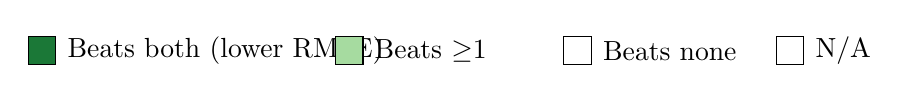
\begin{tikzpicture}[baseline]
\definecolor{both}{HTML}{1B7837}
\definecolor{one}{HTML}{A6DBA0}
\definecolor{none}{HTML}{F4A582}
\node[draw=black,fill=both,minimum width=10pt,minimum height=10pt] at (0,0) {}; \node[anchor=west] at (0.2,0) {Beats both (lower RMSE)};
\node[draw=black,fill=one,minimum width=10pt,minimum height=10pt] at (3.9,0) {}; \node[anchor=west] at (4.1,0) {Beats $\geq$1};
\node[draw=black,fill=none,minimum width=10pt,minimum height=10pt] at (6.8,0) {}; \node[anchor=west] at (7.0,0) {Beats none};
\node[draw=black,fill=white,minimum width=10pt,minimum height=10pt] at (9.5,0) {}; \node[anchor=west] at (9.7,0) {N/A};
\end{tikzpicture}
\caption{Color grid using APE \textbf{RMSE}: x-axis = two-feature combinations, y-axis = sequences. Deep green: combo lower than both singles; light green: lower than at least one; light red: lower than none; white: N/A. Missing single treated as win.}
\label{tab:combo-gain-grid-rmse}
\end{minipage}
\end{table*}